%!TEX program = xelatex
%!TEX root = ...
\documentclass[12pt,hyperref={CJKbookmarks=true}]{beamer}
\usetheme{CambridgeUS}
\usecolortheme{dolphin}
\usefonttheme{professionalfonts}
\setbeamertemplate{bibliography item}{}
\usepackage[noindent]{ctex}%ctex套用英文标题格式(建议在英文论文混排中文时使用),ctexcap套用中文格式(等同于\documentclass{ctexart})
\renewcommand{\figurename}{图}
\renewcommand{\tablename}{表}
\renewcommand{\bibname}{参考文献}
%\renewcommand{\thefigure}{\chinese{figure}}%将图片计数改为汉字数字
%\renewcommand{\thetable}{\chinese{table}}%将表格计数改为汉字数字

\usepackage{amsmath,amssymb,esint}%数学公式类宏包;最末为积分符号拓展
%\numberwithin{equation}{section}%公式编号包含章节
%\usepackage{cite}
\usepackage{bm}%加粗(用于vector)
%\usepackage{textcomp}%符号包,不能用于数学模式,建议不要和SIunits混用
\renewcommand*{\vec}[1]{\bm{#1}}
\usepackage[squaren]{SIunits}%科学单位包,可以用于数学模式(为了统一不要和textcomp混用),squaren选项消除和amssymb的冲突
\usepackage{graphicx}%插图宏包
%\usepackage{picinpar}%图文绕排
\usepackage{array}%表格宏包
%\usepackage{longtable}%长表格宏包
\usepackage{multirow}%多行合并的表格宏包
%\usepackage{booktabs}%表格线宏包
\usepackage{braket}
\usepackage{mathrsfs}%数学字体

%\usepackage[basic,box,gate,oldgate,ic,optics,physics]{circ}%电路图宏包
%\usepackage[normalem]{ulem}%下划线,删除线等宏包,参数表示不修改\emph{}格式
%\usepackage{mychemistry}%化学宏包,包含mhchem和chemfig
%\usepackage[symbol]{footmisc}%脚注拓展,选项表示用符号做脚注记号

%\renewcommand*{\vec}[1]{\bm{#1}}%矢量的格式,这里是加粗
\newcommand{\dif}{\,\mathrm d}
\newcommand\mi{\mathrm{i}}
\newcommand\e{\mathrm{e}}%定义数学模式中常用的正体字符
\newcommand{\Tr}{\operatorname{Tr}}
\newcommand{\St}{{\mathsf{St}}}
\newcommand{\rank}{{\mathsf{rank}}}
\newcommand{\Span}{{\mathsf{Span}}}
\title{信息熵与量子信息熵}
\author{吕铭}
\institute{清华大学物理系}
\date{统计力学课堂报告, 2015}
\begin{document}
\begin{frame}
\titlepage
\end{frame}
\begin{frame}
    \tableofcontents
\end{frame}
\section{Shannon 信息熵} % (fold)
\label{sec:Shannon_entropy}
\subsection{信息熵的来源} % (fold)
\label{ssub:The_concept}
\begin{frame}%[allowframebreaks]
    \frametitle{Shannon 信息熵}
    \begin{itemize}
        \item 动机: 描述一套编码对应的几率分布所包含的信息量\\
        有 $n$ 种可能的状态, 出现的几率分别是 $p_1, p_2, \cdots, p_n$, 希望有一个函数 $H(\vec p)$ 来描述信息量\pause
        \item 要求满足的条件:\\
        三条公理\cite{Shannonentropy}
    \end{itemize}
\end{frame}
\begin{frame}[allowframebreaks]
    \frametitle{Shannon 信息熵}
    三条公理\cite{Shannonentropy}
    \begin{itemize}
        \item 关于 $p_i$ 连续
        \item $p_i = 1/n$ 时, 关于 $n$ 单调增的
        \item 拆分过程应当相当于按权重求和
        \begin{equation}
            H(p_1\vec q_1, p_2\vec q_2, \cdots) = H(\vec p) + \sum p_iH(\vec q_i)
        \end{equation}
    \end{itemize}
    满足上面三条的表达式只能是:
    \begin{equation}
        H(\vec p) = -k\sum_i p_i\log p_i\quad k>0
    \end{equation}
    \begin{proof}
        令 $A(n) = H(1/n,1/n,\cdots,1/n)$, 据第三条公设有
        \begin{equation}
            A(mn) = A(m) + A(n)
        \end{equation}
        同时 $A(n)$ 是单调函数, 从而 $A(n) = k\log n$.

        对于一般的 $\vec p$, 不妨假定 $p_i = n_i/\sum n_i$, 据第三条公设
        \begin{equation}
            k\log\sum n_i = H(\vec p) + \sum p_i k\log n_i
        \end{equation}
        于是 $H = -k\sum p_i\log p_i$, 由单调性和连续性可以推广到实数
    \end{proof}
\end{frame}
% subsubsection The_concept (end)
\begin{frame}
    \frametitle{为什么叫 ``熵''}
    回顾一下课堂内讲到过的熵的微观对应量 (Gibbs 熵)
    $$
        S = -k_B\langle\ln\rho\rangle = -k_B\sum_s\rho_s\ln\rho_s
    $$
    其中 $\rho$ 表示态密度 (不同态的几率分布)\pause

    虽然公式的来源不同但形式完全一致, 这也是为什么将这个量称为熵\footnote{``The form of $H$ will be recognized as that of entropy as defined in certain formulations of statistical mechanics...''\cite{Shannonentropy}}
\end{frame}
\subsection{Shannon 熵的推广: R\'enyi 熵} % (fold)
\label{sub:Renyi_entropy}
\begin{frame}
    \frametitle{Shannon 熵的推广: R\'enyi 熵}
    Alfr\'ed R\'enyi 将这个概念推广到一族函数\cite{renyientropy} :
    \begin{equation}
        H_\alpha(\vec p) = \frac1{1-\alpha}\log\left[\sum_{i=1}^dp_i^\alpha\right]\qquad\alpha\ge 0
    \end{equation}\pause
    Shannon 熵是 $\alpha\to 1$ 时的特例
\end{frame}
\begin{frame}
    \frametitle{信息熵的取值范围}
    \begin{equation}
        0\le H_\alpha(\vec p) \le\log n
    \end{equation}

    上限时 $p_i = \mbox{const.}$ 表示每一种可能的信号都等可能, 
    是信息编码效率最高的情况. (有趣的是, 纯噪音也是这种情况)

    下限时 $p_i = \delta_{ij}$ 表示没有信息, 因为只有一种可能的信号
\end{frame}
% subsection Renyi_entropy (end)
\subsection{信息熵与统计物理} % (fold)
\label{sub:Info_entropy_and_thermo}
\begin{frame}
    \frametitle{信息熵的概念与统计力学}
    \begin{minipage}[t]{0.65\linewidth}
    % 在我们之前讲的统计力学中, 
    % 我们以等几率原理 (equal \textit{a priori} probabilities) 为基本假设出发, 
    % 导出熵作为一个热力学函数来描述热力学关系. 
    % 信息熵的概念使得我们可能以概率论导出熵, 
    % 再根据概率论的最大熵原则导出等几率原理 
    等几率原理 $\Rightarrow$ 热力学关系 $\Rightarrow$ 熵\\
    {\center v.s.}
    熵 $\Rightarrow$ 统计学关系 $\Rightarrow$ 等几率原理 \\
    (Maximum entropy thermodynamics)\pause


    在这个意义下我们并不需要额外的物理学假设来构建统计力学\cite{ITSM.PhysRev.106.620,ITSM2.PhysRev.108.171}.
    % The mere fact that the same mathematical expression $-\sum p\log p$ occurs
    % both in statistical mechanics and in information theory
    % does not in itself establish any connection between
    % these fields. This can be done only by finding new
    % viewpoints from which thermodynamic entropy and
    % information-theory entropy appear as the same \emph{concept}.

    % Previously, one constructed a
    % theory based on the equations of motion, supplemented
    % by additional hypotheses of ergodicity, metric transitivity,
    % or equal \textit{a priori} probabilities, and the identification
    % of entropy was made only at the end, by comparison
    % of the resulting equations with the laws of
    % phenomenological thermodynamics. Now, however, we
    % can take entropy as our starting concept, and the fact
    % that a probability distribution maximizes the entropy
    % subject to certain constraints becomes the essential fact
    % which justifies use of that distribution for inference.

    %II
    % It is of the greatest importance to recognize that in
    % all of this semiclassical theory it is possible to maintain
    % the view that the system is at all times in some definite
    % but unknown pure state, which changes because of
    % definite but unknown external forces; the probabilities
    % represent only our ignorance as to the true state. With
    % such an interpretation the expression ``irreversible
    % process'' represents a semantic confusion; it is not the
    % physical process that is irreversible, but rather our
    % ability to follow it. The second law of thermodynamics
    % then becomes merely the statement that although our
    % information as to the state of a system may be lost in a
    % variety of ways, the only way in which it can be gained
    % is by carrying out further measurements. Essential
    \end{minipage}
    \begin{minipage}[t]{0.3\linewidth}
    \begin{figure}[!ht]
     \centering
     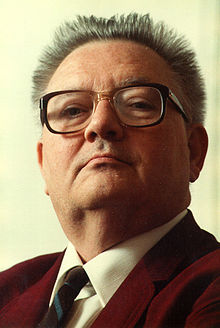
\includegraphics[width=0.8\linewidth]{ETJaynes.jpg}
     \caption{Edwin Thompson Jaynes (1922--1998)}
    \end{figure}
    \end{minipage}
\end{frame}
% subsection Info_entropy_and_thermo (end)
% section 香农信息熵 (end)


\section{量子信息熵} % (fold)
\label{sec:Quantum_entropy}
\begin{frame}
    \tableofcontents[currentsection]
\end{frame}
\subsection{量子态的``混合程度''} % (fold)
\label{sub:Intro_of_quantum_entropy}
\begin{frame}
    \frametitle{对于一个量子态``混合程度''的度量}
    用密度矩阵来表示一个态
    \begin{equation}
        \hat\rho  = \sum_i p_i\ket{\psi_i}\bra{\psi_i}
    \end{equation}\pause
    \begin{definition}
        态 $\hat\rho$ 比态 $\hat\rho'$ ``混合程度''更高, 
        当且仅当存在一组幺正变换 $U_i$ 和概率分布 $p_i$
        \begin{equation}
            \hat\rho = \sum q_k U_k\hat\rho' U_k^\dagger
        \end{equation}
    \end{definition}\pause
    显然对于具有相同本征值组的态, 是具有相当的 ``混合程度'' 的. 
    $$
     \hat\rho' = U\hat\rho U^\dagger\quad U = \sum_i\ket{\psi_i'}\bra{\psi_i}
    $$
    因此概念应当只针对密度矩阵的本征值组
\end{frame}
\begin{frame}[allowframebreaks]
    \frametitle[majorization criterion]{majorization criterion 优化准则}
    \begin{theorem}
        将密度矩阵对角化:
        \begin{equation}
            \hat\rho = \sum_{i=1}^d p_{i}\ket{\alpha_{i}}\bra{\alpha_{i}} 
        \end{equation}
        并且假定本征值排序 $p_{1}\ge p_{2}\ge\cdots\ge p_{d}\ge 0$, 
        则 $\hat\rho$ 比 $\hat\rho'$ 更加``混合''等价于
        \begin{equation}
            \forall t\in\{1,\cdots,d-1\},\qquad \sum_{i=1}^t p_{i}\ge\sum_{i=1}^t p'_{i}
        \end{equation}
        记作 $\vec p \preceq \vec p'$
    \end{theorem}

    \begin{proof}
        \begin{align*}
            \sum_{i=1}^t p'_{i} &= \sum_{i=1}^t \braket{\psi'_i|\hat\rho'|\psi'_i} 
            = \sum_k q_k \sum_{j=1}^d p_j\sum_{i=1}^t |\braket{\psi'_i|U_k|\psi_j}|^2 \\
            &\le \sum_k q_k \sum_{j=1}^t p_j\sum_{i=1}^t|\braket{\psi'_i|U_k|\psi_j}|^2 \\
                &\qquad (\mbox{with }\Span\{U_k\ket{\psi_i}\}_{i=1}^t=\Span\{\ket{\psi'_i}\}_{i=1}^t) \\
            &= \sum_k q_k \sum_{j=1}^t p_j = \sum_{j=1}^t p_j
        \end{align*}
    \end{proof}
\end{frame}
\subsection{混合程度的度量与熵} % (fold)
\label{sub:mixedness_and_entropy}
\begin{frame}
    \frametitle{majorization 的度量}
    \begin{definition}
        Schur-convex: 函数 $f:\mathbb R^d\mapsto\mathbb R$, 
        $\forall \vec x,\vec y\in\mathbb R^d, \vec x\preceq \vec y$, 有 $f(x)<f(y)$ \\
        Schur-concave: $-f$ 是 Schur-convex 的
    \end{definition}\pause
    \begin{definition}[R\'enyi 熵]
        一族的具有 Schur-concave 性质的函数
        \begin{equation}
            H_\alpha(\vec p) = \frac1{1-\alpha}\log\left[\sum_{i=1}^dp_i^\alpha\right]\qquad\alpha\ge 0
        \end{equation}
    \end{definition}
\end{frame}
\begin{frame}
    \frametitle{混合程度的度量}
    直接根据前面的数学定义, 用密度矩阵来表达即为:
    \begin{definition}[量子 R\'enyi 熵]
        定义 $\alpha$ 范数 
        $\Vert\hat\rho\Vert_\alpha := \left(\Tr|\hat\rho^\alpha|\right)^{1/\alpha}$, 
        则量子 R\'enyi 熵的表达式
        \begin{equation}
            S_\alpha(\hat\rho) := \frac{\alpha}{1-\alpha}\log\Vert\hat\rho\Vert_\alpha
        \end{equation}
    \end{definition}
\end{frame}
% subsection mixedness_and_entropy (end)
\begin{frame}
    \frametitle{R\'enyi 熵的性质}
    取值范围
    \begin{equation}
        0\le S_\alpha\le\log d
    \end{equation}\pause

    广延性
    \begin{equation}
        S_\alpha(\hat\rho\otimes\sigma) = S_\alpha(\hat\rho) + S_\alpha(\sigma)
    \end{equation}\pause

    如果将 $\hat \rho$ 视作整个系统所有粒子的密度矩阵 $\rho\in\St[\mathcal H^{\otimes N}]$.
    则这个上限恰为热力学 $S\sim\log\Omega$.
    取最小时当且仅当 $\hat\rho$ 是纯态, 取最大值时当且仅当 $\hat\rho = I/d$
\end{frame}
\begin{frame}
    \frametitle{von-Neumann 熵}
    参照经典信息论的 Shannon 熵, 定义量子 von-Neumann 熵\cite{neumann1932mathematische}
    \begin{equation}
        S(\hat\rho):=\lim_{\alpha\to 1}S_\alpha(\hat\rho) = -\Tr[\hat\rho\log\hat\rho]
    \end{equation}
    这与 Gibbs 熵用密度矩阵的表达式是一致的
\end{frame}
\begin{frame}\frametitle{更``混合''定义的推广}
    \begin{definition}
        $\hat\rho_1\in\mathcal H_1$ 比 $\hat\rho_2\in\mathcal H_2$ 混合程度更高, 
        当且仅当 $\hat\rho_1\otimes\ket\alpha_2\bra\alpha_2$ 比 
        $\ket\beta_1\bra\beta_1\otimes\hat\rho_2$ 混合程度更高
    \end{definition}\pause
    补上纯态对于本征值组来说只是增加了一串 $0$
\end{frame}
\begin{frame}
    \frametitle{von-Neumann 熵的特殊性质}
    特殊的性质, 定义比率 $R$ 为 $\hat\rho^{\otimes N}$ 
    比 $\hat\rho'^{\otimes NR}$ 混合程度更高, 则
    \begin{equation}
        R \le \frac{S(\hat\rho)}{S(\hat\rho')}
    \end{equation}
\end{frame}
% subsection Intro_of_quantum_entropy (end)
% section 密度矩阵与分布函数 (end)

\section{量子信息熵的应用 (举例)} % (fold)
\label{sec:Quantum_info_entropy}
\begin{frame}
    \tableofcontents[currentsection]
\end{frame}
\subsection{粒子的几率分布}
\begin{frame}[allowframebreaks,allowdisplaybreaks]
    \frametitle[关于粒子分布]{从信息熵的观点看粒子分布}
    对于一个 $N$ 粒子体系, 
    单粒子的密度矩阵 (期望) 为 $\hat\rho = \sum q_m\ket{\psi_m}\bra{\psi_m}$, 
    整个体系
    \begin{equation}
        \hat\rho^{\otimes N} = \sum_{\vec m}q_N(\vec m)\ket{\psi_{\vec m}}\bra{\psi_{\vec m}}
    \end{equation}
    其中定义
    \begin{itemize}
        \item $\vec m = (m_1,\cdots, m_N)\in\{1,\cdots,d\}^{\times N}$
        \item $q_N(\vec m)$ 是相应的几率 $q_N(\vec m) = \prod_i q_{m_i}$ 
        \item $\ket{\psi_{\vec m}}$ 是相应的直积态 
        $\ket{\psi_{\vec m}} := \ket{\psi_{m_1}}\ket{\psi_{m_2}}\cdots\ket{\psi_{m_N}}$
    \end{itemize}

    另外定义分布序列
    \begin{equation}
        t_{\vec m}:=(N_1/N,\cdots,N_{d}/N)
    \end{equation}
    于是有:
    \begin{itemize}
        \item 可能的分布总数量 $T_N \sim 1$
        \item 某一中分布 $t$ 对应的态的数量 $S_{N,t} \sim \exp[N H(t)]$ 
        \item 某一组分布 $t$ 出现的几率 $Q_{N,t}\sim \exp[-ND(t\Vert q)]$
    \end{itemize}
\end{frame}

\begin{frame}[allowframebreaks,allowdisplaybreaks]
    \begin{proof}
        可能的分布总数量
        \begin{align*}
            T_N &= \binom{N+d-1}{d-1} \\
            &=\frac{(N+d-1)!}{(d-1)!N!}\\
            &\sim O(N^{d-1})
        \end{align*}
    \end{proof}

    \begin{proof}
        某一组分布中态的数量
        \begin{align*}
            S_{N,t} &= \binom{N}{N_1}\binom{N-N_1}{N_2}\cdots\binom{N_d}{N_d} 
            = \frac{N!}{N_1!N_2!\cdots N_d!} \\
            &\sim \exp\left[N(\ln N - 1) - \sum_{i=1}^d N_i(\ln N_i - 1)\right]\\
            &= \exp\left[N\left(\ln N - \sum_{i=1}^d t_i\ln N_i\right)\right]\\
            &= \exp\left[N H(t_{\vec m})\right]
        \end{align*}
        其中出现了熵的表达式 $H(t_{\vec m}) := -\sum_{i=1}^d t_i\ln t_i$
    \end{proof}

    \begin{proof}
        某一组分布的几率
        \begin{align*}
            Q_{N,t} &= S_{N,t}\prod_{i=1}^dq_i^{N_i} \\
            &\sim\exp\left[N\left(
                \ln N - \sum_{i=1}^d t_i\ln N_i + \sum_{i=1}^d t_i\ln q_i
            \right)\right] \\
            &= \exp[-ND(t\Vert q)]
        \end{align*}
        其中 $D(t\Vert q) := \sum_{i=1}^d t_i\ln\frac{t_i}{q_i}$ 
        称为 Kullback-Leibler(KL) 散度, 也称相对熵\cite{kullback1951information}
    \end{proof}

    从上面的式子还能看出对于偏离 $q_{\vec m}$ 分布的 $t$ 分布是随着粒子数迅速趋于 $0$ 的
    \begin{align*}
        \sum_{t:D(t\Vert q)\ge\epsilon_N} Q_{N,t} 
        &\lesssim \exp[-N\epsilon_N]\sum_{t:D(t\Vert q)\ge\epsilon_N}1\\
        &\le \exp[-N\epsilon_N] T_N \\
        &\sim \exp[-N\epsilon_N]
    \end{align*}
    取$\epsilon_N$ 序列使得 $\lim_{N\to\infty}N\epsilon_N\to\infty$ 即可 
\end{frame}
\subsection{量子纠缠的度量} % (fold)
\label{sub:measure_entanglement}
\begin{frame}
    \frametitle{量子纠缠的度量 (略)}
    如果定义``更纠缠''为``不可以通过局域操作 
    (LOCC\footnote{Local operations and classical communication}) 
    转化'', 那么可以证明前面关于``更混合''的定义与``更纠缠''有关联
    \begin{theorem}
        $\ket\Psi\bra\Psi$ 更纠缠当且仅当 $\Tr_B[\ket\Psi\bra\Psi]$ 更混合
    \end{theorem}
    特别的, Bell 态 $\ket{\Psi^\pm}$ 是最大纠缠态, 
    它的部分迹是完全混合态 $\Tr_B[\ket{\Psi^\pm}\bra{\Psi^\pm}] = I/2$
\end{frame}
% subsection measure_entanglement (end)
\subsection{量子信息的压缩} % (fold)
\label{sub:Quantum_compression}
\begin{frame}[allowframebreaks]
    \frametitle{量子信息的压缩 (略)}
    定义量子通道 (quantum channel) $\mathscr C(\rho) = \Tr_B[U(\rho\otimes\sigma)U^\dagger]$, 
    存在一组量子量子通道编码方案 $\mathscr E:\mathcal H_d\mapsto\mathcal H_{d'}$ 
    与相应的解码方案 $\mathscr D:\mathcal H_{d'}\mapsto\mathcal H_d$ (其中 $d'<d$)
    使得以 $p_i$ 的几率编码为量子态 $\ket{\psi_i}$ 的量子信息 (可以描述为密度矩阵)
    经过编码和解码后几乎不变
    $$
    \Vert\rho - \mathscr D\mathscr E(\rho)\Vert_1<\epsilon
    $$
    \begin{theorem}[Schumacher’s noiseless channel coding theorem]
        在 $N\to\infty$ 渐进意义下, 对于 $\rho^N$ 信号的压缩
        $\mathscr E:\mathcal H_{2^N}\mapsto\mathcal H_{d_N}$ 以及
        $\mathscr D:\mathcal H_{d_N}\mapsto\mathcal H_{2^N}$, 定义压缩率
        \begin{equation}
            R := \limsup_{N\to\infty}\frac{\log d_N}{N}
        \end{equation}
        理论可以达到的最佳压缩率为 $R\ge S(\rho)$\cite{noisecodeing.PhysRevA.51.2738}
    \end{theorem}
\end{frame}
% subsection Quantum_compression (end)
% section 量子信息熵 (end)
\section{参考文献} % (fold)
\label{sec:参考文献}
\begin{frame}[allowframebreaks]
    \frametitle{参考文献}
    \bibliographystyle{apalike}
    \bibliography{aboutentropy}
\end{frame}
% section 参考文献 (end)
\end{document}